1. Diseñar una función transferencia que cumpla con las especificaciones.
2. Diseñar un circuito que implemente la función transferencia utilizando un Gyrator. Justificar adecuadamente la elección de todos sus componentes y redactar una introducción teórica al tema.
3. Determinar rangos de operación en zona lineal. Se espera adecuada profundidad en este análisis.
4. Contrastar el diseño del circuito con las simulaciones correspondientes.
5. Implementar el circuito y comprobar su funcionamiento con las mediciones correspondientes.
6. Analizar el comportamiento del sistema en altas frecuencias.
7. Diseñar un PCB que contenga todos los circuitos pedidos (en el mismo PCB). A su vez, puede utilizarse un
sólo IC en la implementación pedida.

En la presente sección, se implementarán cuatro filtros de segundo orden según las siguientes especificaciones:

\begin{table}[H]
    \centering
    \begin{tabular}{|c|c|c|c|}
    \hline
    \rowcolor[HTML]{C0C0C0} 
    Tipo de Filtro & $f_p[Hz]$ & $f_a[Hz]$ & $f_c[Hz]$ \\ \hline
    Low-Pass       & 5000   & 17500  & -      \\ \hline
    High-Pass      & 21000   & 6000   & -      \\ \hline
    Band-Pass      & -      & -      & 10000  \\ \hline
    Band-Rejection & -      & -      & 6000   \\ \hline
    \end{tabular}
    \end{table}

En los casos Low-Pass y High-Pass se espera también:

\begin{itemize}
	\item Ganancia mayor a -3 dB cuando $f < f_p$ o $f > f_p$ 
	\item Ganancia menor a -10 dB cuando $f > f_a$ o $f < f_a$
	\item Ganancia nunca superior a 0 dB
	\item Ganancia unitaria en continua ($f \to \infty$)
\end{itemize}

Cada circuito será empleado implementando una resistencia $R$, una inductancia $L$ y un capacitor $C$, es decir un circuito $RLC$
clásico. 

La inductancia $L$ será reemplazada por componentes que unidos presenten un comportamiento similar a ella, en este caso
un Gyrator. 

Antes de introducirnos en el diseño de filtros propiamente, se realizará una introducción a este elemento que se utilizará para observar
por qué es tan útil y por qué lo emplearemos para las experiencias reemplazando la inductancia.

\subsubsection{Introducción a Gyrators}

Un Gyrator o girador es considerado un elemento pasivo adicional a los ya conocidos y analizados. Una de sus tantas funcionalidades es ser empleado como un inductor. 
El motivo de reemplazar a un inductor real por este dispositivo, se encuentra en fines prácticos, ya que al utilizar éste en lugar de una inductancia, se pueden reducir 
tanto el tamaño de un circuito como el costo del mismo. 

Una inductancia tiene asociada una resistencia que por lo general no podremos controlar. El cable que se utiliza para elaborar una inductancia tiene dicha resistencia asociada. 
Por otro lado, se pueden obtener capacitores de alta calidad y con un girador, por ende, obtener inductores de alta calidad y a su vez, pudiendo manipular el valor de la resistencia asociada.

Un gyrator puede ser empleado de diferentes maneras. En el presente trabajo, nos focalizaremos en el gyrator compuesto por un amplificador operacional, dos resistencias y un capacitor.
Es importante saber que se puede definir también al gyrator como un inversor de las características corriente voltaje de un componente eléctrico.

El símbolo circuital utilizado para el gyrator es el siguiente:

\begin{figure}[H]
    \centering
    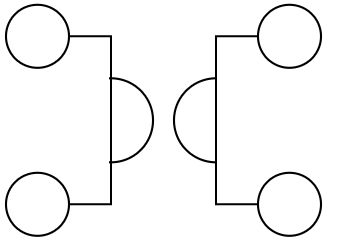
\includegraphics[width=0.25\textwidth]{../Ejercicio2-DiseñoDeFiltros/Imagenes/diagrama-basico-gyrator.png}
    \caption{Símbolo circuital del Gyrator}
\end{figure}

\subsubsection{Implementación real de un Gyrator}

En la cátedra se han demostrado diferentes formas de implementarlo incluso con dos amplificadores, pero con el fin de simplificar las mediciones
y armado de los distintos filtros se analizará el caso con un solo amplificador y se focalizará la atención en cómo lograr que éste se comporte como un 
inductor.

En el siguiente diagrama se puede ver la implementación de un Gyrator como un inductor observando éste a la izquierda y su equivalente a la derecha:

\begin{figure}[H]
    \centering
    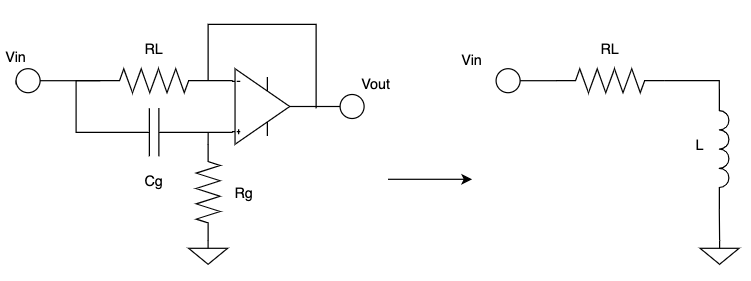
\includegraphics[width=0.6\textwidth]{../Ejercicio2-DiseñoDeFiltros/Imagenes/diagrama-gyrator-inductor.png}
    \caption{Equivalente circuital entre Gyrator e Inductor}
\end{figure}

En la próxima sección se verá que este equivalente no es válido para todo el rango de frecuencias, sino que su comportamiento dependerá de 
determinadas condiciones. El gyrator actuará como un inductor cuasi ideal hasta determinadas frecuencias donde su comportamiento 
como tal se deteriorará, factores en los cuales el amplificador operacional toma gran parte.

\subsubsection{Análisis de $Z_{in}$}

Para describir el comportamiento del circuito como un inductor es importante 
analizar la impedancia de entrada a dicho circuito tal que $Z_{in}=\frac{V_{in}}{I_{in}}$. 
Para ello, utilizaremos el siguiente diagrama circuital:

\begin{figure}[H]
    \centering
    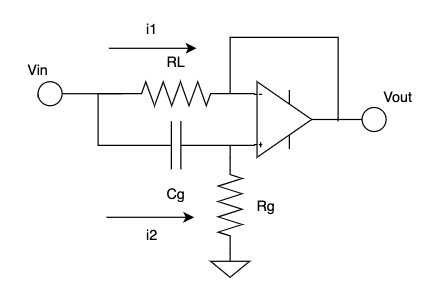
\includegraphics[width=0.4\textwidth]{../Ejercicio2-DiseñoDeFiltros/Imagenes/diagrama-gyrator-corrientes.png}
    \caption{Diagrama de Gyrator como Inductor}
\end{figure}

Se puede observar del gráfico que:

$$V_{out}=V^-$$

Por ello:

$$V_{out}=A_{vol}(V^+-V^-) \longrightarrow V^-=A_{vol}(V^+-V^-) 
\longrightarrow V^-= V^+ \frac{A_{vol}}{1+A_{vol}}$$

Utilizando un divisor de tensión, obtenemos la siguiente relación:

$$V^+= V_{in}\frac{R_g}{R_g+\frac{1}{SC_g}}$$

Por definición en el diagrama anterior:

$$I_{in}=i_1+i_2$$

Como no ingresa corriente al amplificador operacional, definimos a las corrientes como:

$$i_1=\frac{V_{in}-V^-}{R_L}$$
$$i_2=\frac{V^+}{R_g}$$

Entonces:

$$I_{in}=\frac{V_{in}-V^-}{R_L}+\frac{V^+}{R_g} \longrightarrow 
I_{in}=V_{in}(\frac{R_g+\frac{1}{SC_g}+R_L-R_g\frac{A_{vol}}{1+A_{vol}}}{R_L(R_g+\frac{1}{SC_g})})$$

Finalmente:

$$Z_{in}=\frac{V_{in}}{I_{in}}=\frac{V_{in}}{V_{in}(\frac{R_g+\frac{1}{SC_g}+R_L-R_g\frac{A_{vol}}{1+A_{vol}}}{R_L(R_g+\frac{1}{SC_g})})} \longrightarrow
Z_{in}=\frac{R_L(R_g+\frac{1}{SC_g})}{R_g+\frac{1}{SC_g}+R_L-R_g\frac{A_{vol}}{1+A_{vol}}}$$

Si ahora multiplicamos por el factor $SC_g$ en numerador y denominador:

$$Z_{in}=\frac{R_L(SC_gR_g+1)}{SC_g(R_g+R_L-R_g\frac{A_{vol}}{1+A_{vol}})+1}$$

Como $A_{vol}=\frac{A_0}{1+\frac{S}{w_p}}$, el factor $\frac{A_{vol}}{1+A_{vol}}$ cambia su comportamiento
según la frecuencia de trabajo:

$$\frac{A_{vol}}{1+A_{vol}}=\frac{\frac{A_0}{1+\frac{S}{w_p}}}{1+\frac{A_0}{1+\frac{S}{w_p}}}=
\frac{A_0}{A_0+1+\frac{S}{w_p}}=\frac{1}{1+\frac{1}{A_0}+\frac{S}{A_0w_p}}$$

Notemos que $GBP$ o el Gain Bandwidth Product es equivalente a $A_0w_p$, y $A_0$ tiene un valor alto, por ello se puede aproximar la anterior
expresión a:

$$\frac{1}{1+\frac{S}{GBP}}$$

Siempre que $1 >> \frac{S}{GBP}$ , podremos aproximar dicha expresión:

$$\frac{1}{1+\frac{S}{GBP}} \approx 1$$

Obteniendo así una impedancia de entrada con una forma que se acerca a un inductor real:

$$Z_{in}=\frac{R_L(sC_gR_g+1)}{sC_gR_L+1}$$

Tomaremos dicha relación cuando $\frac{S}{GBP} \geq 10$, o equivalente a decir una diferencia de un orden de magnitud.

Caso contrario, nuestro impedancia no podrá aproximarse a un inductor y el comportamiento no será el esperado así que aquí se presenta 
una primera condición.

Como $Z_{in}=\frac{R_L(SC_gR_g+1)}{SC_gR_L+1}$, para obtener una expresión de la forma de un inductor,
podremos establecer otra relación necesaria tal que:

$$1 >> SC_gR_L$$

Cumpliendo dicha condición, nuestro inductor usando gyrator estará representado por:

$$Z_{in}=R_L(sC_gR_g+1)\longrightarrow Z_{in}=sC_gR_gR_L+R_L$$

Donde:

$$L=C_gR_gR_L$$

Como nota final de este comportamiento es importante ver que la relación $1 >> SC_gR_L$, se cumplirá a bajas frecuencias,
mayores o menores dependiendo de los componentes elegidos. Además de ello, el Gyrator para ser empleado como inductor en este caso deberá estar
referenciado a tierra aunque en uno de los filtros a diseñar se lo implementará de tal manera que esté flotante. Luego se podrán observar las limitaciones
tanto por los polos del amplificador operacional como por el rango de trabajo como inductor del gyrator propuesto. 


Nuestro equivalente quedará representado por:

\begin{figure}[H]
    \centering
    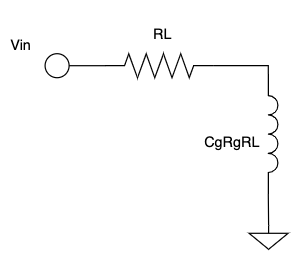
\includegraphics[width=0.3\textwidth]{../Ejercicio2-DiseñoDeFiltros/Imagenes/equivalente-inductor.png}
    \caption{Equivalente de Inductor utilizando un Gyrator}
\end{figure}

\subsubsection{Elección del amplificador operacional para el Gyrator}

Para la implementación experimental del Gyrator y de los distintos filtros, 
se ha elegido el circuito integrado $TL084$, cuya hoja de datos se puede encontrar \href{https://www.ti.com/lit/ds/symlink/tl084.pdf?ts=1602260789397&ref_url=https%253A%252F%252Fwww.ti.com%252Fproduct%252FTL084}{aquí} por diferentes razones:

\begin{itemize}
	\item Al momento de armar el PCB contaremos con 4 amplificadores operacionales en un solo circuito integrado, ideal para el diseño de 4 filtros con 1 gyrator cada uno. 
	\item Slew-Rate típico de $13 \frac{V}{\mu s}$ lo cual nos permitirá trabajar experimentalmente en un amplio rango sin sufrir alinealidad en el comportamiento de los filtros.
	\item GBP típico de $3MHz$ , por lo cual nuestra relación $1 >> \frac{S}{GBP}$ se cumplirá para un gran rango de frecuencias.
\end{itemize}

\subsection{Filtro Pasa-Bajos (Low-Pass)}

Se procederá a realizar un filtro pasa-bajos de segundo orden clásico, tal que podemos
ver la disposición de elementos en la siguiente figura:

\begin{figure}[H]
    \centering
    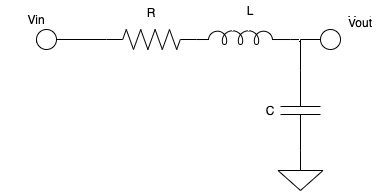
\includegraphics[width=0.5\textwidth]{../Ejercicio2-DiseñoDeFiltros/Imagenes/diagrama-pasa-bajos.png}
    \caption{Circuito Pasa-Bajos de segundo orden con elementos pasivos}
\end{figure}

Las especificaciones son las siguientes:

\begin{itemize}
	\item E1: Ganancia mayor a -3 dB cuando $f < 5 KHz$ 
	\item E2: Ganancia menor a -10 dB cuando $f > 17.5 KHz $
	\item E3: Ganancia nunca superior a 0 dB
	\item E4: Ganancia unitaria en continua ($f \to \infty$)
\end{itemize}

En el dominio de Laplace podemos ver que la función de transferencia para este circuito está dada por:

$$H(S)=\frac{V_{out}(S)}{V_{in}(S)}=\frac{\frac{1}{SC}}{SL+R+\frac{1}{SC}} \longrightarrow 
H(S)=\frac{1}{S^2LC+SCR+1}$$

De allí podemos observar que $w_0=\frac{1}{\sqrt{LC}}$, $Q=\frac{1}{2\xi}$ y $\xi=\frac{R\sqrt{C}}{2\sqrt{L}}$.

Por la condición E3, la ganancia nunca deberá superar a 0 dB entonces en otras palabras no se deben presentar sobrepicos en el circuito RLC.
Sabiendo que los sobrepicos se presentarán en casos donde $\xi \leq \frac{1}{\sqrt{2}}$, se tomarán valores que cumplan la relación:

$$\xi > \frac{1}{\sqrt{2}}$$.

Además de ello, para un circuito de segundo orden la pendiente de la recta que se presenta en $H(S)$ es de 
40 $\frac{dB}{dec}$, más precisamente -40 $\frac{dB}{dec}$ en este caso. 

Para establecer una relación y hallar una frecuencia de corte $f_0$ apropiada, 
sabiendo que en valores un poco anteriores a dicha frecuencia, la pendiente se empieza a notar,y tal que se cumplan los requisitos
de la plantilla, E1 y E2, estableceremos una diferencia mínima de 10 dB entre $5 KHz$ y $17.5 KHz$, ya que la diferencia establecida por la plantilla
es de por lo menos 7 dB (-3 dB a -10 dB) para dichas frecuencias y buscaremos la relación entre las dos frecuencias para que una vez establecida la $f_0$,
obtengamos el comportamiento deseado.

Sabiendo que en $\frac{1}{4}$ de década se representará una diferencia de 10 dB para dicha función transferencia, buscando obtener una
relación entre ambas frecuencias según lo estipulado previamente y estableciendo la condición E2 para obtener la relación:

$$\frac{1}{4}=\log_{10}(\frac{17.5KHz}{f_0})$$

De esta manera, podremos estimar una $f_0$ tal que se cumpla la plantilla:

$$f_0 = \frac{17.5KHz}{1.7782} = 9.84 KHz$$

Se esperará que antes de dicha frecuencia la ganancia esté por encima de los $-3dB$, por ende se cumplirá la condición E1. 
Por ello y para trabajar con frecuencias enteras, se utilizará una frecuencia un poco menor, $f_0=9 KHz$ ya que con la diferencia establecida de 10 dB, 
usar una frecuencia menor, no afectará el comportamiento esperado según la plantilla y todavía nos encontraremos en los límites estipulados.

Por las relaciones expresadas previamente:

$$w_0=\frac{1}{\sqrt{LC}} \longrightarrow 2\pi f_0=\frac{1}{\sqrt{LC}}$$

Luego:

$$\frac{R\sqrt{C}}{2\sqrt{L}} > \frac{1}{\sqrt{2}}$$

Como tenemos varias incógnitas, elegiremos el $C$ a utilizar basándonos en los elementos disponibles, siendo para este caso,
$C=0.1\mu F$.

Por ello:

$$2\pi 9KHz=\frac{1}{\sqrt{L0.1 \mu F}} \longrightarrow L = 3.1271 mH$$

Además:

$$\frac{R\sqrt{0.1\mu F}}{2\sqrt{3.1271mH}} > \frac{1}{\sqrt{2}} \longrightarrow R > 249.76 \Omega $$

Es importante notar que a medida que $R$ aumenta nos encontraremos en una situación donde el circuito será
cada vez más sobreamortiguado, y por ello buscaremos utilizar un valor de $R$ lo más cercano posible al calculado teóricamente, ya que de otra forma
por la reducción de la pendiente debido al sobreamortiguamiento podríamos no encontrarnos en los parámetros establecidos en la plantilla. 
Se utilizó entonces $R= 330 \Omega$ ya que es el valor más cercano con el que se contaba.


\begin{table}[H]
    \centering
    \begin{tabular}{|c|c|c|}
    \hline
    \rowcolor[HTML]{C0C0C0} 
    R[$\Omega$] & C[$\mu F$] & L[$mH$]  \\ \hline
    330      & 0.1  & 3.1271 \\ \hline
    \end{tabular}
    \end{table}

Una vez obtenidos los valores nominales de los elementos, se buscó implementar dicho circuito pero utilizando el gyrator descripto previamente
para reemplazar a la inductancia. Para ello, basándonos 
en las siguientes relaciones:

$$Z=sC_gR_gR_L+R_L$$

$$1 >> sC_gR_L$$

Partiendo de la última expresión, se escogió:

\begin{table}[H]
    \centering
    \begin{tabular}{|c|c|c|l|}
    \hline
    \rowcolor[HTML]{C0C0C0} 
    $R_L[\Omega]$ & $C_g[\mu F$] & $R_g[\Omega]$  & $L_{eq}[mH]$ \\ \hline
     10       & 0.1  & 3300 & 3.3        \\ \hline
    \end{tabular}
    \end{table}


Notar que el valor escogido es tal que $C=C_g$ y $R_L$ es pequeña en comparación a la $R$ del circuito para no generar
un sobreamortiguamiento adicional.

Se verifica a continuación el rango de frecuencias de trabajo:

$$1 >> (S0.1 \mu )(10) \longrightarrow 1  >> 2 \pi f 10^{-6}$$

Se procedió a simular el comportamiento del circuito RLC equivalente con los valores obtenidos de la implementación con el 
gyrator para observar si su comportamiento es el esperado:

\begin{table}[H]
    \centering
    \begin{tabular}{|c|c|c|}
    \hline
    \rowcolor[HTML]{C0C0C0} 
    $R+R_L[\Omega]$ & C[$\mu F$] & L[$mH$]  \\ \hline
    340      & 0.1  & 3.3 \\ \hline
    \end{tabular}
    \end{table}

\begin{figure}[H]
    \centering
    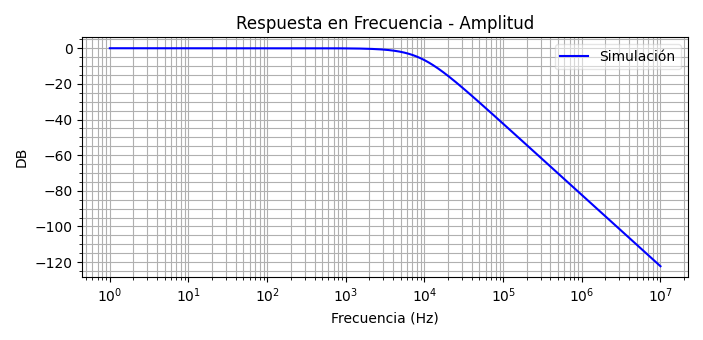
\includegraphics[width=0.6\textwidth]{../Ejercicio2-DiseñoDeFiltros/Imagenes/bode-rlc-pasa-bajos-amplitud.png}
    \caption{Circuito Pasa-Bajos de segundo orden}
\end{figure}

\begin{figure}[H]
    \centering
    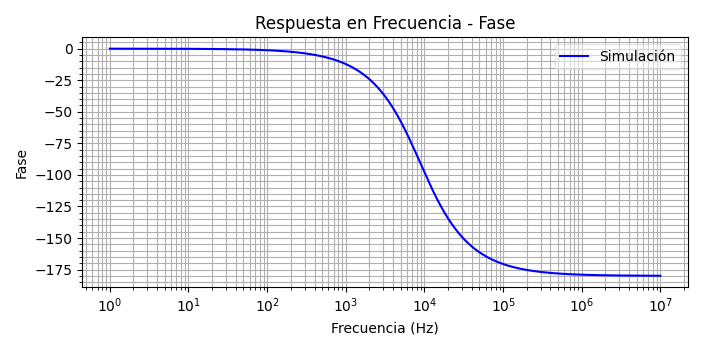
\includegraphics[width=0.6\textwidth]{../Ejercicio2-DiseñoDeFiltros/Imagenes/bode-rlc-pasa-bajos-fase.png}
    \caption{Circuito Pasa-Bajos de segundo orden}
\end{figure}

Se pudo comprobar entonces que para el circuito equivalente con gyrator se cumple lo establecido en la plantilla.
De la simulación se observó que en $f=5.00007 KHz$, la ganancia es de $-1.904 dB$ y en $f=17.503KHz$, es de $-13.25 dB$

Comprobado ello, se realizó la simulación utilizando ahora el amplificador operacional y los elementos pasivos del gyrator obtenidos anteriormente.

\begin{figure}[H]
    \centering
    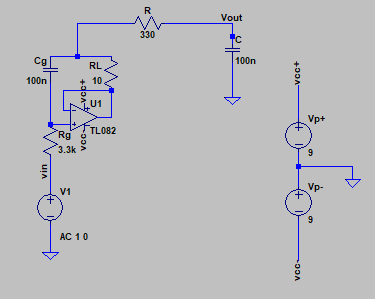
\includegraphics[width=0.5\textwidth]{../Ejercicio2-DiseñoDeFiltros/Imagenes/pasa-bajos-opamp-diagrama.png}
    \caption{Circuito Pasa-Bajos de segundo orden}
\end{figure}

Lo obtenido fue lo siguiente:

\begin{figure}[H]
    \centering
    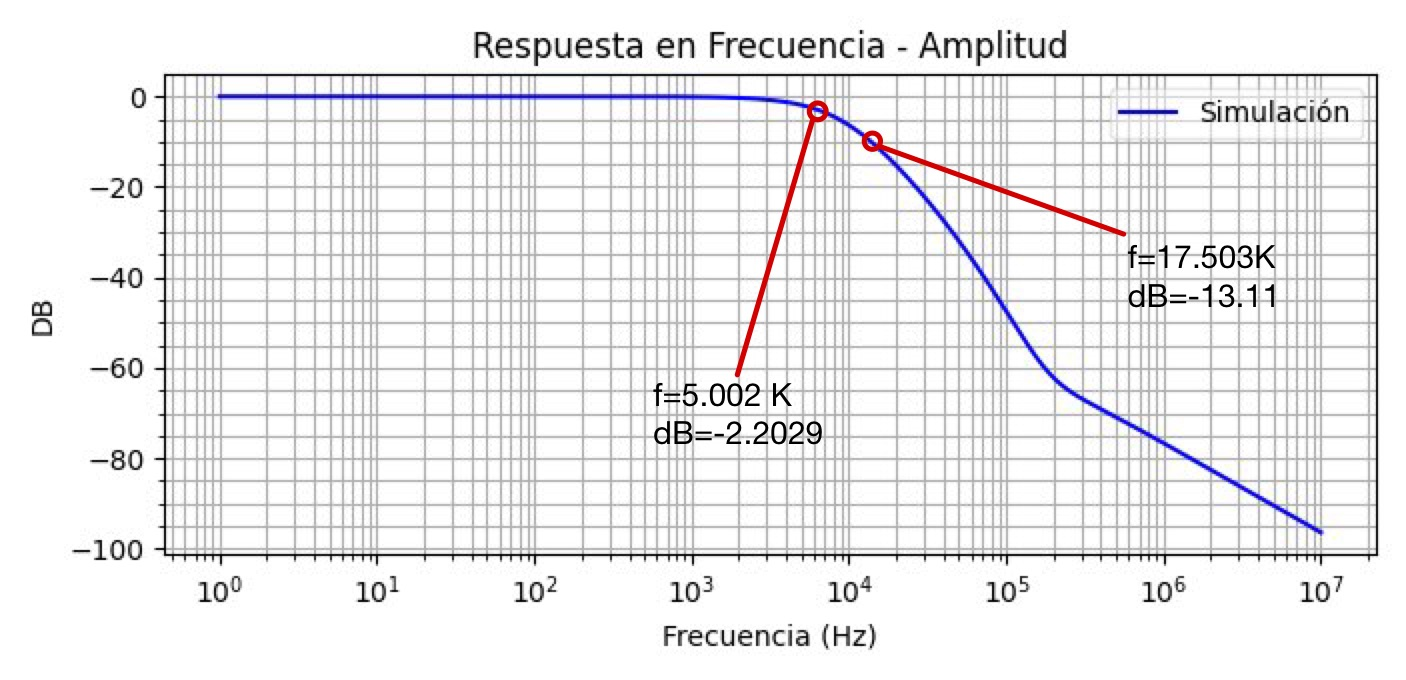
\includegraphics[width=0.7\textwidth]{../Ejercicio2-DiseñoDeFiltros/Imagenes/Pasa-Bajos-Marcado-Opamp.jpg}
    \caption{Circuito Pasa-Bajos de segundo orden}
\end{figure}

\begin{figure}[H]
    \centering
    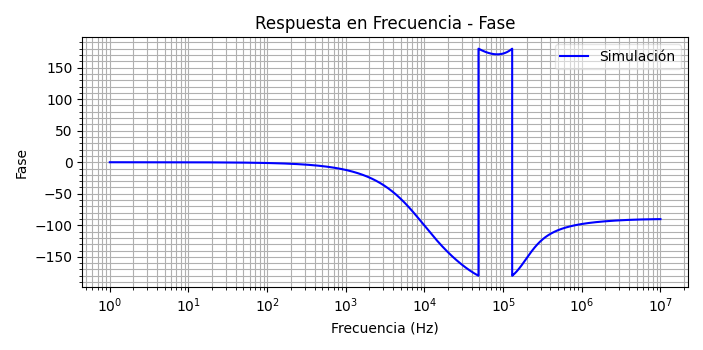
\includegraphics[width=0.7\textwidth]{../Ejercicio2-DiseñoDeFiltros/Imagenes/bode-opamp-pasa-bajos-fase.png}
    \caption{Circuito Pasa-Bajos de segundo orden}
\end{figure}

Se puede comprobar aquí también que la plantilla se sigue cumpliendo obteniendo el filtro pasa-bajos con el comportamiento deseado.

Como punto final, se empleó el circuito diseñado en la $Digital$ $Explorer$ $Board$, y se midió la respuesta en frecuencia:

\begin{figure}[H]
    \centering
    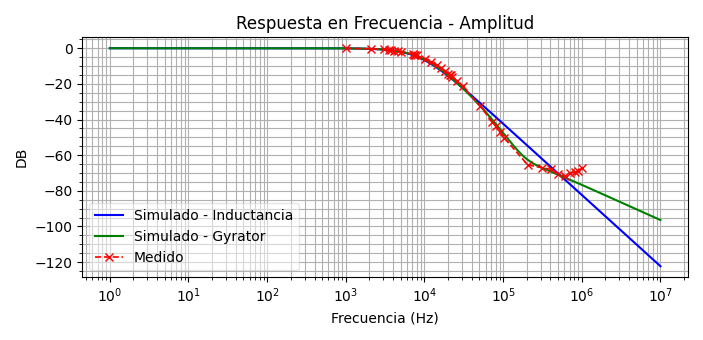
\includegraphics[width=0.6\textwidth]{../Ejercicio2-DiseñoDeFiltros/Imagenes/pasa-bajos-final-amplitud.png}
    \caption{Circuito Pasa-Bajos de segundo orden}
\end{figure}

\begin{figure}[H]
    \centering
    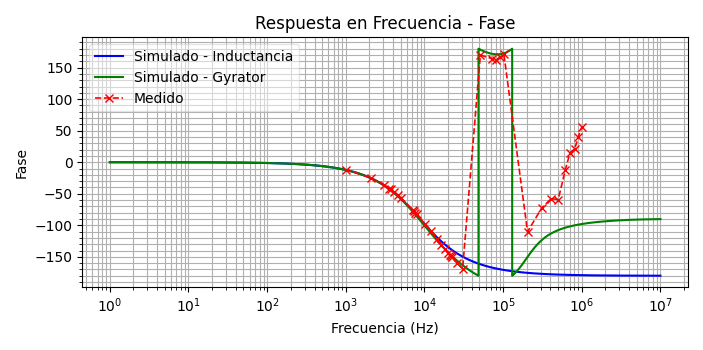
\includegraphics[width=0.6\textwidth]{../Ejercicio2-DiseñoDeFiltros/Imagenes/pasa-bajos-final-fase.png}
    \caption{Circuito Pasa-Bajos de segundo orden}
\end{figure}

\subsection{Filtro Pasa-Altos (High-Pass)}

Se realizó un filtro pasa-altos de segundo orden clásico, tal que podemos
ver la disposición de elementos para el mismo en la siguiente figura:

\begin{figure}[H]
    \centering
    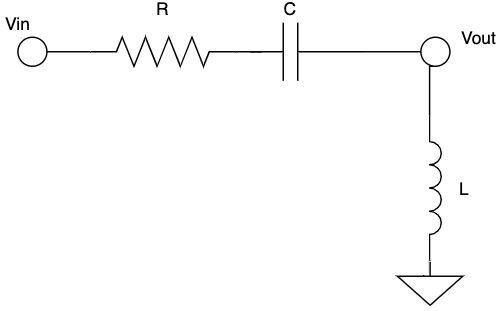
\includegraphics[width=0.5\textwidth]{../Ejercicio2-DiseñoDeFiltros/Imagenes/diagrama-pasa-altos.png}
    \caption{Circuito Pasa-Altos de segundo orden}
\end{figure}

Las especificaciones para esta experiencia son las siguientes:

\begin{itemize}
	\item E1: Ganancia mayor a -3 dB cuando $f > 21 KHz$ 
	\item E2: Ganancia menor a -10 dB cuando $f < 6 KHz $
	\item E3: Ganancia nunca superior a 0 dB
	\item E4: Ganancia unitaria en continua ($f \to \infty$)
\end{itemize}

En el dominio de Laplace podemos ver que la función de transferencia para este circuito está dada por:

$$H(S)=\frac{V_{out}(S)}{V_{in}(S)}=\frac{SL}{SL+R+\frac{1}{SC}} \longrightarrow H(S)=\frac{S^{2}LC}{S^2LC+SRC+1}$$

Aquí también podemos observar que $w_0=\frac{1}{\sqrt{LC}}$, $Q=\frac{1}{2\xi}$ y $\xi=\frac{R\sqrt{C}}{2\sqrt{L}}$.

Como la ganancia nuevamente nunca deberá superar a 0 dB no se deberán presentar sobrepicos en este circuito.
Sabiendo que los sobrepicos se presentarán también aquí en casos donde $\xi \leq \frac{1}{\sqrt{2}}$, se tomarán valores que cumplan la relación:

$$\xi > \frac{1}{\sqrt{2}}$$.

Se realizará el mismo análisis que para el circuito pasa-bajos, donde para establecer una relación y hallar una frecuencia de corte $f_0$ apropiada, tal que se cumplan los requisitos
de esta plantilla, estableceremos una diferencia mínima de 10 dB entre $21 KHz$ y $6 KHz$, ya que la diferencia establecida por la plantilla, E1 y E2,
es de por lo menos 7 dB (-3 dB a -10 dB).

Mediante dicha relación, entonces sabiendo que en $\frac{1}{4}$ de década se obtendrá una diferencia de 10 dB y tomando como referencia 
la $f$ de E1:

$$\frac{1}{4}=\log_{10}(\frac{21KHz}{f_0})$$

También podremos estimar una $f_0$ tal que se cumpla la plantilla:

$$f_0 = \frac{21KHz}{1.7782} = 11.80 KHz$$

Se utilizará una frecuencia un poco menor, $f_0=11 KHz$ ya que con la diferencia establecida de 10 dB, usar una frecuencia menor, no afectará el comportamiento 
esperado según la plantilla.

Por las relaciones expresadas previamente:

$$w_0=\frac{1}{\sqrt{LC}} \longrightarrow 2\pi f_0=\frac{1}{\sqrt{LC}}$$

Luego:

$$\frac{R\sqrt{C}}{2\sqrt{L}} > \frac{1}{\sqrt{2}}$$

Tomando nuevamente $C$ a utilizar como $C=0.1\mu F$: 

$$2\pi 11KHz=\frac{1}{\sqrt{L0.1 \mu F}} \longrightarrow L = 2.0934 mH$$

Además:

$$\frac{R\sqrt{0.1\mu F}}{2\sqrt{2.0934mH}} > \frac{1}{\sqrt{2}} \longrightarrow R > 204.58 \Omega $$

Otra vez a medida que $R$ aumenta nos encontraremos en una situación donde el circuito será
cada vez más sobreamortiguado, obteniendo efectos no contemplados en los cálculos precedentes. 
Por ello se utilizó un valor de $R= 220 \Omega$ ya que es el valor más cercano con el que se contaba.

\begin{table}[H]
    \centering
    \begin{tabular}{|c|c|c|}
    \hline
    \rowcolor[HTML]{C0C0C0} 
    R[$\Omega$] & C[$\mu F$] & L[$mH$]  \\ \hline
    220     & 0.1  & 2.0934 \\ \hline
    \end{tabular}
    \end{table}

Para implementar dicho circuito pero utilizando el gyrator descripto previamente
para reemplazar a la inductancia y teniendo las relaciones descriptas anteriormente:

$$Z=sC_gR_gR_L+R_L$$

$$1 >> sC_gR_L$$

Partiendo de la última expresión, se escogió:

\begin{table}[H]
    \centering
    \begin{tabular}{|c|c|c|l|}
    \hline
    \rowcolor[HTML]{C0C0C0} 
    $R_L[\Omega]$ & $C_g[\mu F$] & $R_g[\Omega]$  & $L_{eq}[mH]$ \\ \hline
    10      & 0.1  & 2200 & 2.2        \\ \hline
    \end{tabular}
    \end{table}

El valor escogido es tal que $C=C_g$ y $R_L$ es pequeña en comparación a la $R$ del circuito para no generar
un sobreamortiguamiento adicional.

Aquí el rango de trabajo ideal del inductor al haber elegidos los mismos valores de $R_L$ y $C_g$

$$1 >> (S0.1 \mu )(10) \longrightarrow 1  >> 2 \pi f 10^{-6}$$

Se procedió a simular el comportamiento del circuito RLC equivalente con el gyrator implementado para observar si su comportamiento es el esperado:

\begin{table}[H]
    \centering
    \begin{tabular}{|c|c|c|}
    \hline
    \rowcolor[HTML]{C0C0C0} 
    $R+R_L[\Omega]$ & C[$\mu F$] & L[$mH$]  \\ \hline
    230      & 0.1  & 2.2 \\ \hline
    \end{tabular}
    \end{table}

\begin{figure}[H]
    \centering
    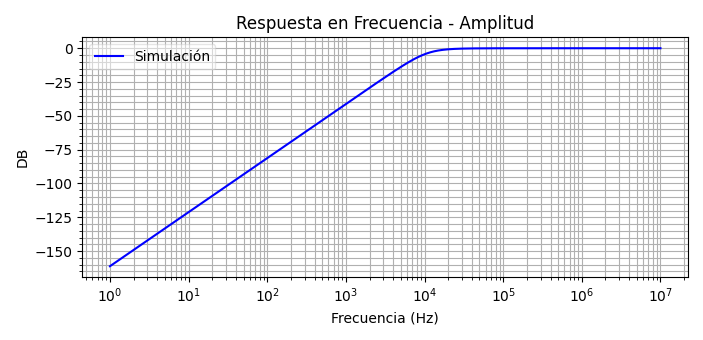
\includegraphics[width=0.6\textwidth]{../Ejercicio2-DiseñoDeFiltros/Imagenes/bode-rlc-pasa-altos-amplitud.png}
    \caption{Circuito Pasa-Bajos de segundo orden}
\end{figure}

\begin{figure}[H]
    \centering
    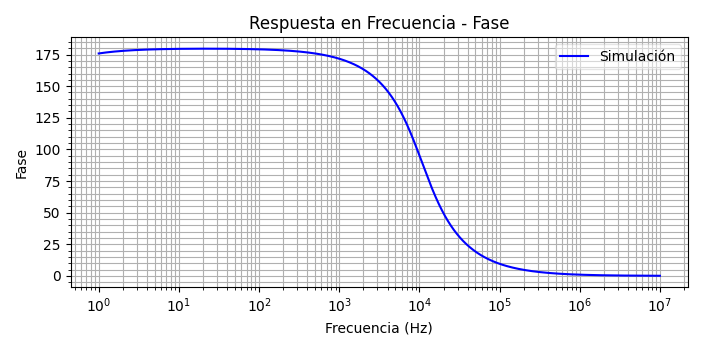
\includegraphics[width=0.6\textwidth]{../Ejercicio2-DiseñoDeFiltros/Imagenes/bode-rlc-pasa-altos-fase.png}
    \caption{Circuito Pasa-Bajos de segundo orden}
\end{figure}

Para el circuito equivalente con gyrator se cumple lo establecido en la plantilla.
De la simulación se observó que en $f=6.00007 KHz$, la ganancia es de $-10.97 dB$ y en $f=21.003KHz$, es de $-0.6955 dB$.

Luego, se realizó la simulación utilizando ahora el amplificador operacional y los elementos pasivos del gyrator obtenidos anteriormente.

\begin{figure}[H]
    \centering
    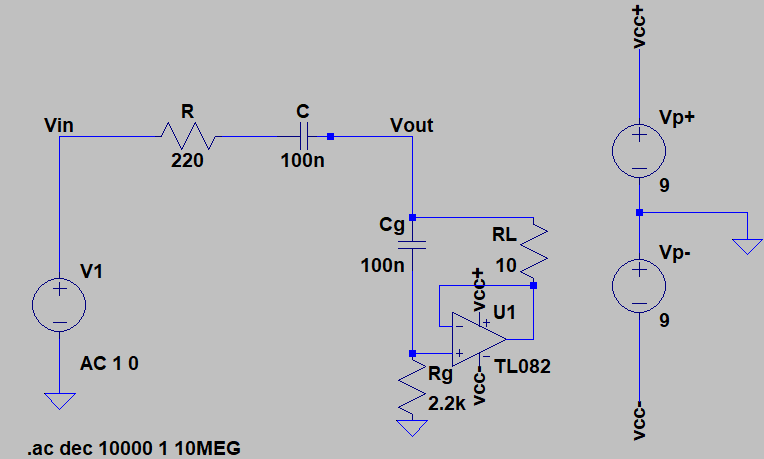
\includegraphics[width=0.4\textwidth]{../Ejercicio2-DiseñoDeFiltros/Imagenes/pasa-altos-opamp-diagrama.png}
    \caption{Circuito Pasa-Bajos de segundo orden}
\end{figure}

Lo obtenido fue lo siguiente:

\begin{figure}[H]
    \centering
    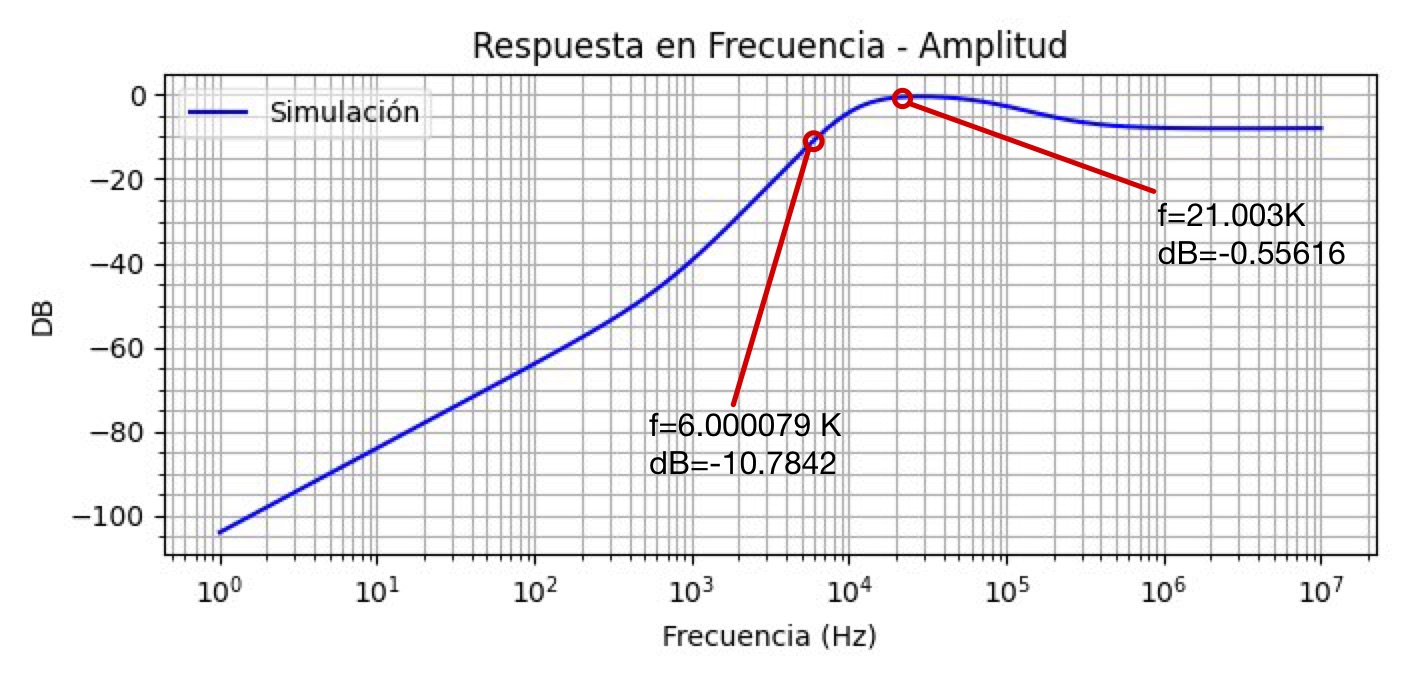
\includegraphics[width=0.6\textwidth]{../Ejercicio2-DiseñoDeFiltros/Imagenes/Pasa-Altos-Marcado-Opamp.jpg}
    \caption{Circuito Pasa-Bajos de segundo orden}
\end{figure}

\begin{figure}[H]
    \centering
    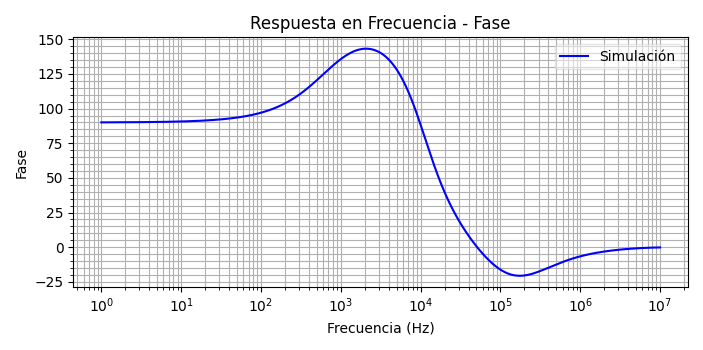
\includegraphics[width=0.6\textwidth]{../Ejercicio2-DiseñoDeFiltros/Imagenes/bode-opamp-pasa-altos-fase.png}
    \caption{Circuito Pasa-Bajos de segundo orden}
\end{figure}

Se puede comprobar aquí también que la plantilla se sigue cumpliendo obteniendo el filtro pasa-altos buscado.

Para contrastar aquí empíricamente, también se armó el circuito en la $Electronics$ $Explorer$ $Board$ y se midió la respuesta
en frecuencia:

\begin{figure}[H]
    \centering
    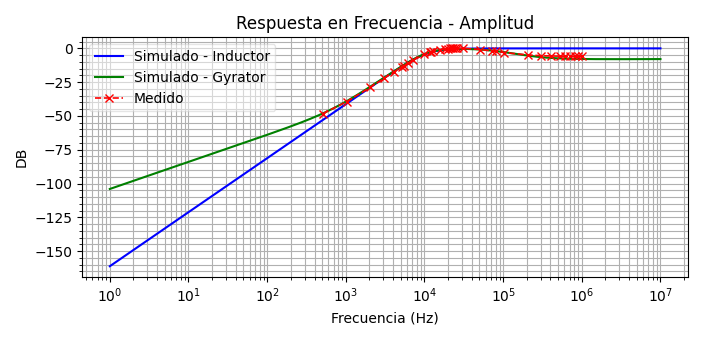
\includegraphics[width=0.6\textwidth]{../Ejercicio2-DiseñoDeFiltros/Imagenes/pasa-altos-final-amplitud.png}
    \caption{Circuito Pasa-Bajos de segundo orden}
\end{figure}

\begin{figure}[H]
    \centering
    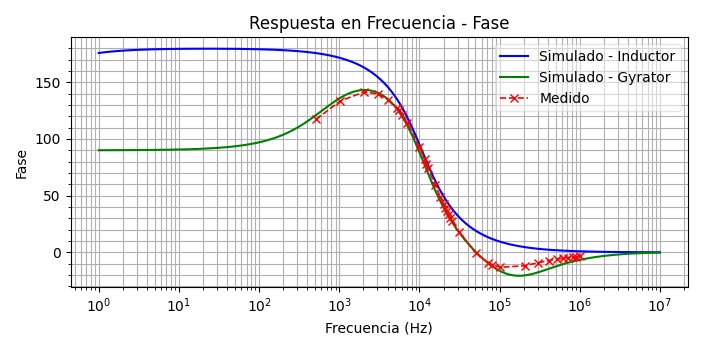
\includegraphics[width=0.6\textwidth]{../Ejercicio2-DiseñoDeFiltros/Imagenes/pasa-altos-final-fase.png}
    \caption{Circuito Pasa-Bajos de segundo orden}
\end{figure}



\subsection{Filtro Rechaza-Banda (Band-Rejection)}

Se procederá a realizar un circuito rechaza-banda de segundo orden clásico, tal que podemos
ver la disposición de elementos en la siguiente figura:

\begin{figure}[H]
    \centering
    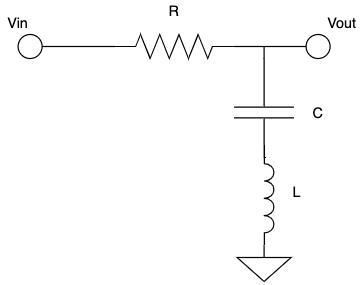
\includegraphics[width=0.4\textwidth]{../Ejercicio2-DiseñoDeFiltros/Imagenes/diagrama-rechaza-banda.png}
    \caption{Circuito Rechaza-Banda de segundo orden}
\end{figure}

La única especificación en este caso es:

\begin{itemize}
	\item E1: $f_c=6 KHz$
\end{itemize}

En el dominio de Laplace podemos observar que la función de transferencia para este circuito es:

$$H(S)=\frac{V_{out}(S)}{V_{in}(S)}=\frac{SL+\frac{1}{SC}}{SL+R+\frac{1}{SC}} \longrightarrow H(S)=\frac{S^{2}LC+1}{S^2LC+SRC+1}$$

Podemos ver que aquí también $w_0=\frac{1}{\sqrt{LC}}$, y por ello:

$$2 \pi f_0 = \frac{1}{\sqrt{LC}} \longrightarrow 2 \pi 6KHz = \frac{1}{\sqrt{LC}}$$

Mantendremos una consistencia en el capacitor utilizado, eligiendo nuevamente $C=0.1 \mu F$, entonces:

$$L = 7.036 mH$$

Para este caso, optaremos por obtener un circuito críticamente amortiguado o cercano a él, por ello utilizando la relación que también aplica a este
filtro:

$$\xi=\frac{R \sqrt{C}}{2\sqrt{L}}=\frac{1}{\sqrt{2}} \longrightarrow R=375.06$$

El valor comercial más cercano con el que contamos es $560 \Omega$ por lo que observaremos un comportamiento sobreamortiguado aunque aquí
no tendrá mucha importancia ya que no se especificaron parámetros adicionales más que E1.

\begin{table}[H]
    \centering
    \begin{tabular}{|c|c|c|}
    \hline
    \rowcolor[HTML]{C0C0C0} 
    R[$\Omega$] & C[$\mu F$] & L[$mH$]  \\ \hline
    560     & 0.1  & 7.036 \\ \hline
    \end{tabular}
    \end{table}

Al analizar el comportamiendo del inductor mediante Gyrator, se obtuvieron los siguientes valores:

\begin{table}[H]
    \centering
    \begin{tabular}{|c|c|c|l|}
    \hline
    \rowcolor[HTML]{C0C0C0} 
    $R_L[\Omega]$ & $C_g[\mu F$] & $R_g[\Omega]$  & $L_{eq}[mH]$ \\ \hline
    10      & 0.1  & 6800 & 6.8        \\ \hline
    \end{tabular}
    \end{table}

Cuyo rango de trabajo se dará también siempre y cuando:

$$1 >> (S0.1 \mu )(10) \longrightarrow 1  >> 2 \pi f 10^{-6}$$

Se procedió a simular el comportamiento del circuito RLC equivalente para observar su comportamiento:

\begin{table}[H]
    \centering
    \begin{tabular}{|c|c|c|}
    \hline
    \rowcolor[HTML]{C0C0C0} 
    $R+R_L[\Omega]$ & C[$\mu F$] & L[$mH$]  \\ \hline
    570      & 0.1  & 6.8 \\ \hline
    \end{tabular}
    \end{table}

\begin{figure}[H]
    \centering
    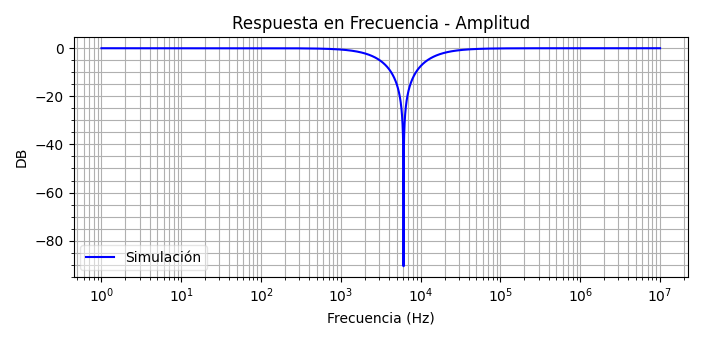
\includegraphics[width=0.6\textwidth]{../Ejercicio2-DiseñoDeFiltros/Imagenes/bode-rlc-rechaza-banda-amplitud.png}
    \caption{Circuito Pasa-Bajos de segundo orden}
\end{figure}

\begin{figure}[H]
    \centering
    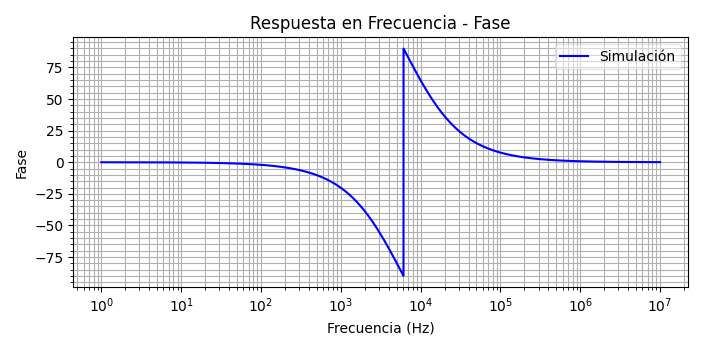
\includegraphics[width=0.6\textwidth]{../Ejercicio2-DiseñoDeFiltros/Imagenes/bode-rlc-rechaza-banda-fase.png}
    \caption{Circuito Pasa-Bajos de segundo orden}
\end{figure}

Se comprobó que para el circuito equivalente con gyrator se cumple lo establecido en la plantilla.
De la simulación se observó que en $f_c=6.1031 KHz$, donde la ganancia es de $-90.64 dB$.

Una vez comprobado el correcto funcionamiento del filtro, se realizó la simulación pertinente al circuito
con el gyrator:

\begin{figure}[H]
    \centering
    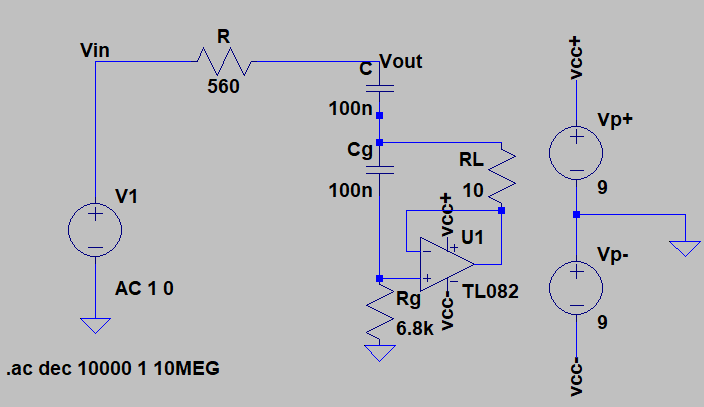
\includegraphics[width=0.5\textwidth]{../Ejercicio2-DiseñoDeFiltros/Imagenes/rechaza-banda-opamp-diagrama.png}
    \caption{Circuito Pasa-Bajos de segundo orden}
\end{figure}

Lo obtenido fue lo siguiente:

\begin{figure}[H]
    \centering
    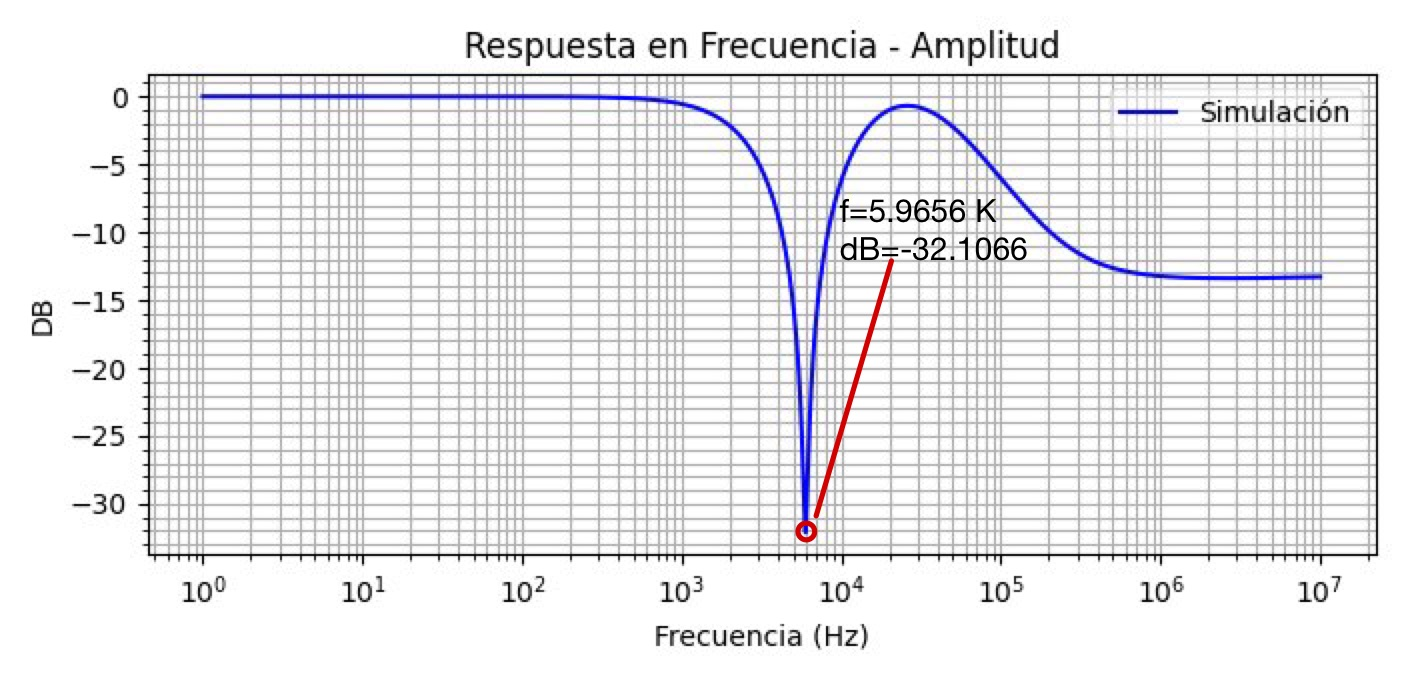
\includegraphics[width=0.7\textwidth]{../Ejercicio2-DiseñoDeFiltros/Imagenes/Rechaza-Banda-Marcado-Opamp.jpg}
    \caption{Circuito Pasa-Bajos de segundo orden}
\end{figure}

\begin{figure}[H]
    \centering
    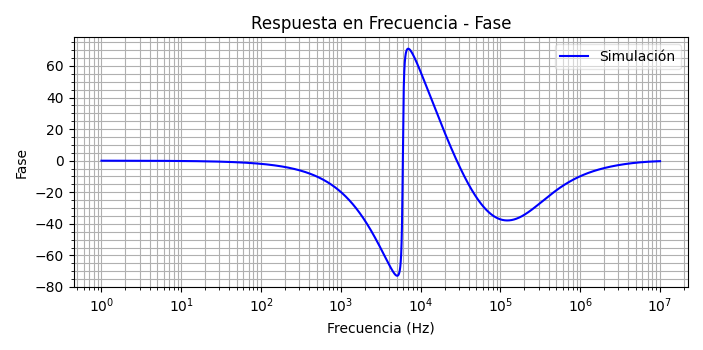
\includegraphics[width=0.7\textwidth]{../Ejercicio2-DiseñoDeFiltros/Imagenes/bode-opamp-rechaza-banda-fase.png}
    \caption{Circuito Pasa-Bajos de segundo orden}
\end{figure}

Se puede comprobar aquí también que la plantilla se sigue cumpliendo obteniendo el filtro rechaza-banda solicitado.

Se procedió a armar el circuito en la $Electronics$ $Explorer$ $Board$, para medir la respuesta en frecuencia del filtro:

\begin{figure}[H]
    \centering
    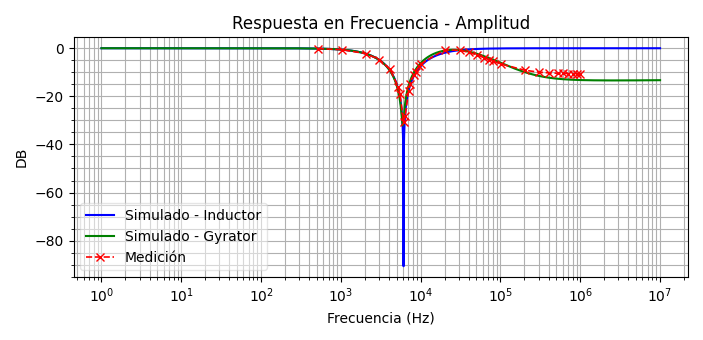
\includegraphics[width=0.7\textwidth]{../Ejercicio2-DiseñoDeFiltros/Imagenes/rechaza-banda-final-amplitud.png}
    \caption{Circuito Pasa-Bajos de segundo orden}
\end{figure}

\begin{figure}[H]
    \centering
    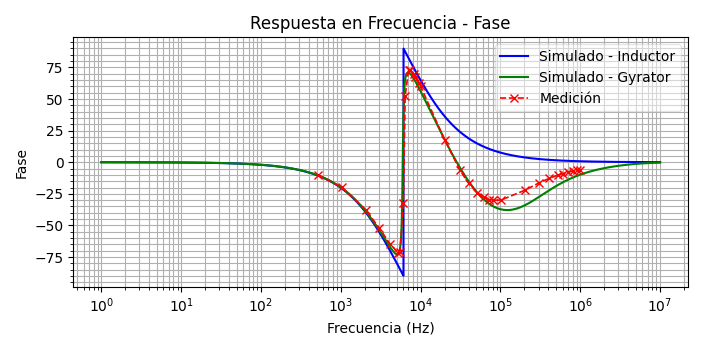
\includegraphics[width=0.7\textwidth]{../Ejercicio2-DiseñoDeFiltros/Imagenes/rechaza-banda-final-fase.png}
    \caption{Circuito Pasa-Bajos de segundo orden}
\end{figure}


\subsection{Filtro Pasa-Banda (Band-Pass)}

Realizaremos como último filtro, un pasa-banda de segundo orden clásico, con los siguientes elementos:

\begin{figure}[H]
    \centering
    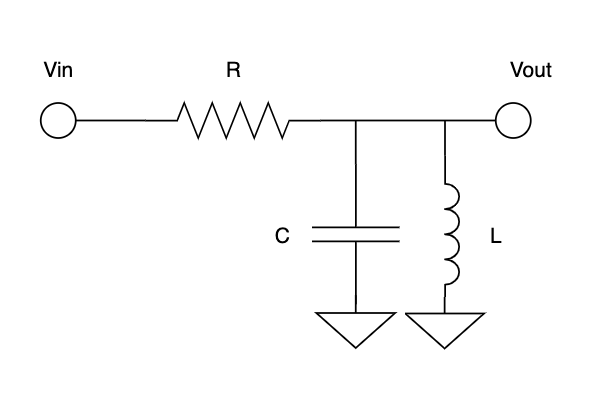
\includegraphics[width=0.5\textwidth]{../Ejercicio2-DiseñoDeFiltros/Imagenes/diagrama-pasa-banda.png}
    \caption{Circuito Pasa-Altos de segundo orden}
\end{figure}

La única especificación en este caso es:

\begin{itemize}
	\item E1: $f_c=10 KHz$
\end{itemize}

Nuevamente utilizando la transformada de Laplace obtenemos la función de transferencia para el último filtro
a diseñar:

$$H(S)=\frac{V_{out}(S)}{V_{in}(S)}=\frac{\frac{1}{SC}\parallel SL}{\frac{1}{SC}\parallel SL + R} \longrightarrow 
H(S)=\frac{S\frac{L}{R}}{S^2LC+S\frac{L}{R}+1}$$

Como en los filtros analizados anteriormente, la frecuencia de corte
será $w_0=\frac{1}{\sqrt{LC}}$, por lo tanto:

$$2 \pi f_0 = \frac{1}{\sqrt{LC}} \longrightarrow 2 \pi 10KHz = \frac{1}{\sqrt{LC}}$$

En todos los filtros optamos por $C=0.1 \mu F$. El mismo será empleado aquí también, por lo que nuestra inductancia será:

$$L = 2.533 mH$$

También al buscar un circuito críticamente amortiguado:

$$\xi=\frac{R \sqrt{C}}{2\sqrt{L}}=\frac{1}{sqrt{2}} \longrightarrow R=225.04$$

El valor que utilizaremos entonces es $220 \Omega$ por lo que observaremes un comportamiento apenas subamortiguado.
Nuevamente no es un factor que nos afecte en el diseño del filtro, ya que la única condición establecida es la frecuencia
de corte.

\begin{table}[H]
    \centering
    \begin{tabular}{|c|c|c|}
    \hline
    \rowcolor[HTML]{C0C0C0} 
    R[$\Omega$] & C[$\mu F$] & L[$mH$]  \\ \hline
    220     & 0.1  & 2.533 \\ \hline
    \end{tabular}
    \end{table}

Para el gyrator, se escogieron los siguientes elementos:

\begin{table}[H]
    \centering
    \begin{tabular}{|c|c|c|l|}
    \hline
    \rowcolor[HTML]{C0C0C0} 
    $R_L[\Omega]$ & $C_g[\mu F$] & $R_g[\Omega]$  & $L_{eq}[mH]$ \\ \hline
    10      & 0.1  & 2700 & 2.7        \\ \hline
    \end{tabular}
    \end{table}

El rango de trabajo del inductor con gyrator es el mismo que para los tres filtros anteriores.

Se simuló el comportamiento del circuito RLC equivalente para verificar el correcto funcionamiento del filtro.

\begin{table}[H]
    \centering
    \begin{tabular}{|c|c|c|}
    \hline
    \rowcolor[HTML]{C0C0C0} 
    $R+R_L[\Omega]$ & C[$\mu F$] & L[$mH$]  \\ \hline
    230     & 0.1  & 2.7 \\ \hline
    \end{tabular}
    \end{table}


\begin{figure}[H]
    \centering
    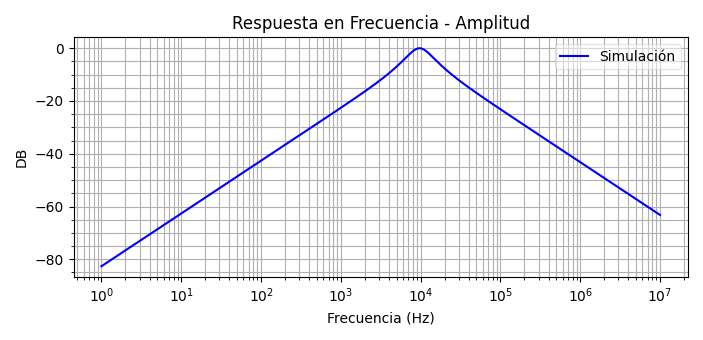
\includegraphics[width=0.6\textwidth]{../Ejercicio2-DiseñoDeFiltros/Imagenes/bode-rlc-pasa-banda-amplitud.png}
    \caption{Circuito Pasa-Bajos de segundo orden}
\end{figure}

\begin{figure}[H]
    \centering
    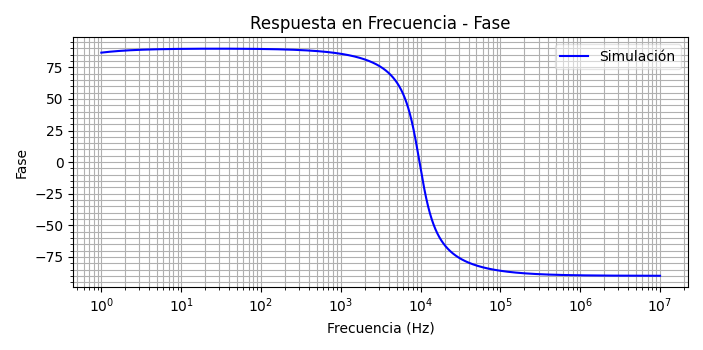
\includegraphics[width=0.6\textwidth]{../Ejercicio2-DiseñoDeFiltros/Imagenes/bode-rlc-pasa-banda-fase.png}
    \caption{Circuito Pasa-Bajos de segundo orden}
\end{figure}

A simple vista se puede observar que la frecuencia de corte es muy cercana a los $10 KHz$

Se realizó la simulación utilizando ahora el amplificador operacional y los elementos pasivos del gyrator obtenidos anteriormente.

\begin{figure}[H]
    \centering
    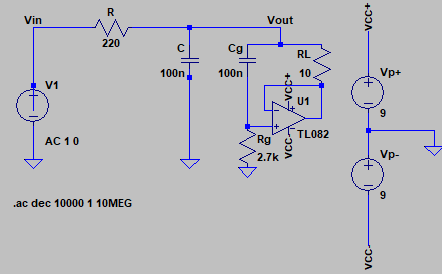
\includegraphics[width=0.5\textwidth]{../Ejercicio2-DiseñoDeFiltros/Imagenes/pasa-banda-opamp-diagrama.png}
    \caption{Circuito Pasa-Bajos de segundo orden}
\end{figure}

Lo obtenido fue lo siguiente:

\begin{figure}[H]
    \centering
    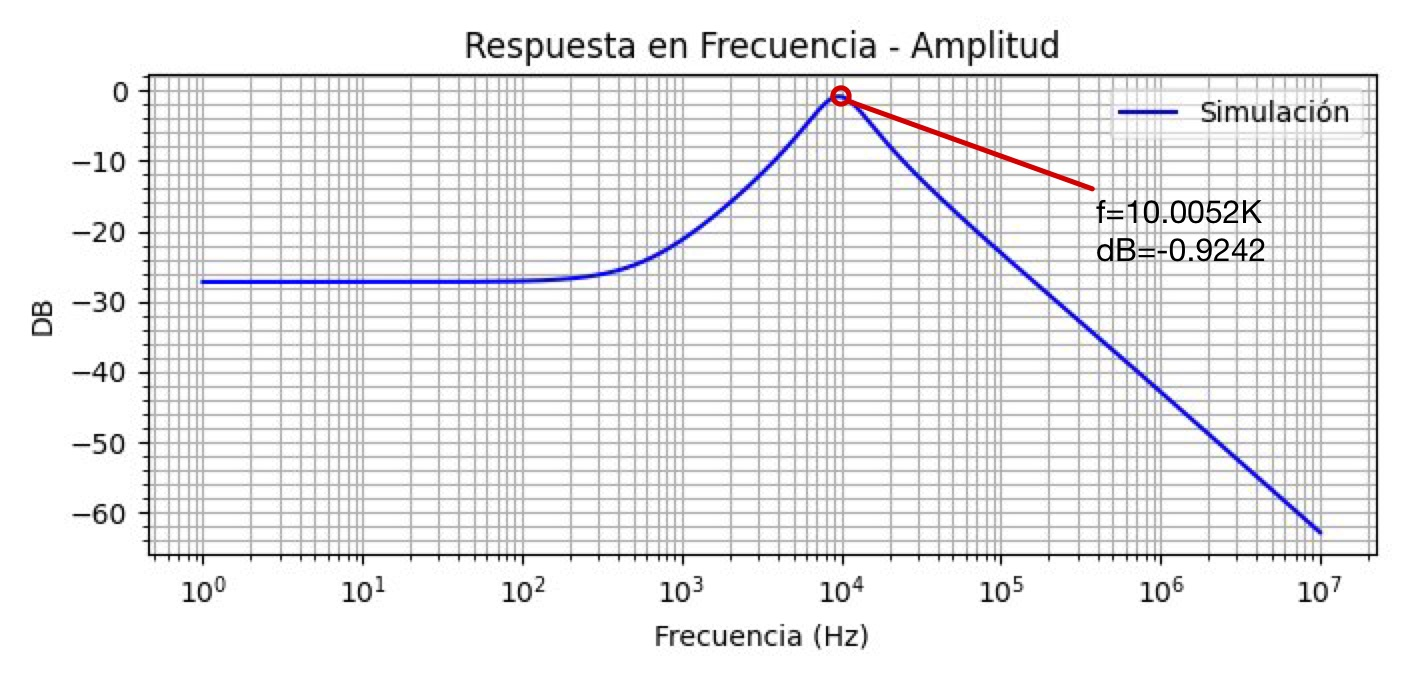
\includegraphics[width=0.7\textwidth]{../Ejercicio2-DiseñoDeFiltros/Imagenes/Pasa-Banda-Marcado-Opamp.jpg}
    \caption{Circuito Pasa-Bajos de segundo orden}
\end{figure}

\begin{figure}[H]
    \centering
    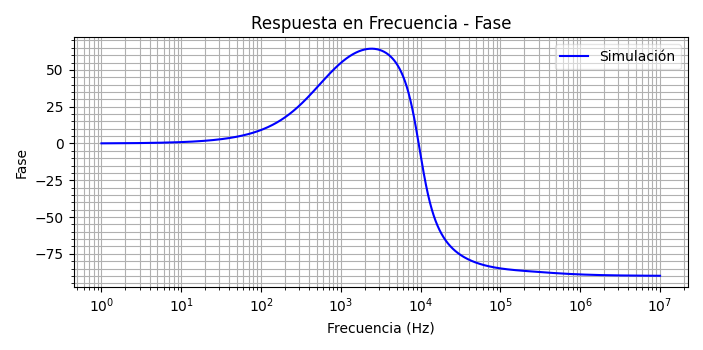
\includegraphics[width=0.7\textwidth]{../Ejercicio2-DiseñoDeFiltros/Imagenes/bode-opamp-pasa-banda-fase.png}
    \caption{Circuito Pasa-Bajos de segundo orden}
\end{figure}

Se puede comprobar aquí también que la plantilla se sigue cumpliendo obteniendo el filtro pasa-banda buscado.

Se procedió a armar el circuito en la $Electronics$ $Explorer$ $Board$, para medir la respuesta en frecuencia:

\begin{figure}[H]
    \centering
    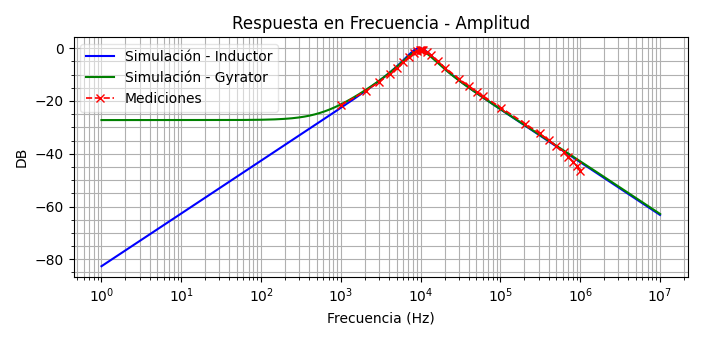
\includegraphics[width=0.7\textwidth]{../Ejercicio2-DiseñoDeFiltros/Imagenes/pasa-banda-final-amplitud.png}
    \caption{Circuito Pasa-Bajos de segundo orden}
\end{figure}

\begin{figure}[H]
    \centering
    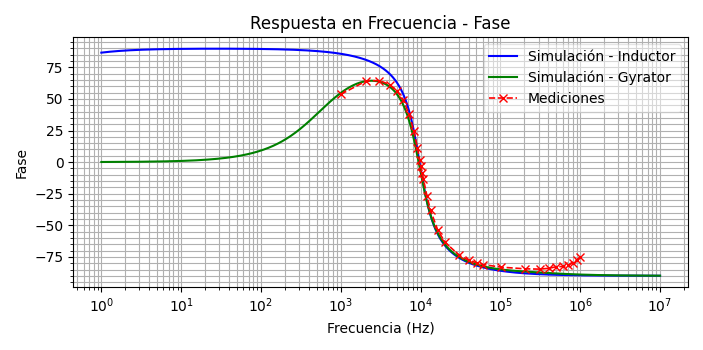
\includegraphics[width=0.7\textwidth]{../Ejercicio2-DiseñoDeFiltros/Imagenes/pasa-bandaa-final-fase.png}
    \caption{Circuito Pasa-Bajos de segundo orden}
\end{figure}

\subsection{Implementación}
En esta sección se plantean las consideraciones de diseño llevadas a cabo para implementar los circuitos presentados anteriormente 
en un PCB. Lamentablemente, dadas las condiciones presentes no se puede implementar físicamente lo expuesto pero se toman todos los 
recaudos necesarios para lograr un diseño fidedigno a una implementación real. \par 

La cátedra plantea la condición de que es necesario implementar el diseño de los filtros usando un sólo circuito integrado, por ende, se 
decide utilizar el $TL084CN$ fabricado por \textit{Texas Instruments},
 encapsulado que cuenta con cuatro amplificadores operacionales en su interior. A su vez, de lo anterior se desprende que habrá que implementar 
 nuestro diseño en el mismo PCB.
Consecuentemente, los cuatro filtros solicitados, \textit{Band Pass}, \textit{Band Reject}, \textit{Low Pass} y \textit{High Pass}, requieren un 
filtro de segundo orden RLC para cumplir con las especificaciones, utilizando un \textit{girator} cada uno para simular una inductancia. Para 
implementar el anterior dispositivo se utiliza el circuito presentado anteriormente en las simulaciones. \par 

\subsubsection{Consideraciones de diseño}
Dado que cada filtro requiere un amplificador operacional y que los valores de inductancia simulados con el girator son distintos para cada implementación,
se considera que lo óptimo es asignar un amplificador operacional a cada filtro, de manera de tener cuatro circuitos implementados en
 la misma placa pero que no comparten 
componentes. De esta manera, se minimiza la posibilidad de errores o de incompatibilidades. \par 

Por otro lado, en vista de un uso óptimo, se procede a aislar los cuatro circuitos para poder usarlos de manera independiente. Esto se logra implementando 
tanto pines a la entrada como a la salida del PCB, los cuales son la conexión eléctrica de entrada y de salida de cada filtro. Se utiliza un 
\textit{header 4x2} en el esquemático que representa las tiras de pares de pines con las conexiones posibles. Para utilizar un filtro es necesario cerrar
 la conexión eléctricamente entre los dos pines utilizando un \textit{jumper}. Este procedimiento se debe realizar tanto a la entrada como a la salida de 
 cada filtro.  Por otro lado, en las proximidades de las conexiones de salida se colocaron dos pines, conectados a la señal de salida y tierra,
  de manera tal de colocar de manera sencilla y práctica la punta del osciloscopio para medir.

\begin{figure}
      
 \centering
 \begin{subfigure}[b]{0.33\textwidth}
     \centering
     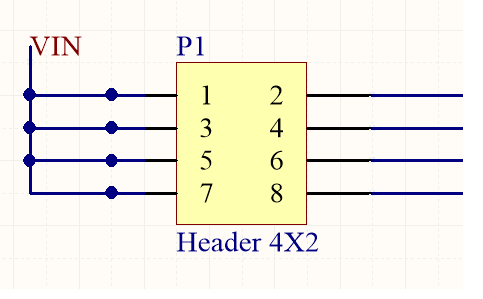
\includegraphics[width=\textwidth]{../Ejercicio2-DiseñoDeFiltros/Imagenes/esquematico_pines_in.png}
     \caption{Implementación a nivel esquemático}
 \end{subfigure}
 \hfill
 \begin{subfigure}[b]{0.33\textwidth}
     \centering
     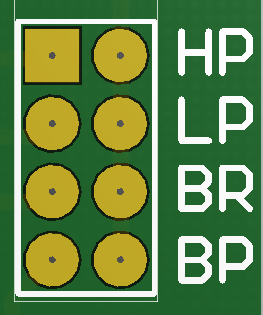
\includegraphics[width=\textwidth]{../Ejercicio2-DiseñoDeFiltros/Imagenes/esquematico_pines_out.png}
     \caption{Implementación a nivel PCB}
 \end{subfigure}
 \hfill
 \begin{subfigure}[b]{0.33\textwidth}
    \centering
    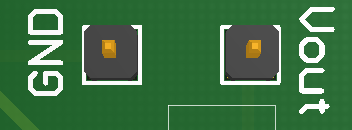
\includegraphics[width=\textwidth]{../Ejercicio2-DiseñoDeFiltros/Imagenes/esquematico_pines_sal.png}
    \caption{Implementación punto de medición}
\end{subfigure}
\end{figure}

La limitación que nos plantea este diseño es la imposibilidad de medir más de un filtro a la vez. A nivel lógico lo implementado responde al siguiente 
esquema:

\begin{figure}[H]
    \centering
    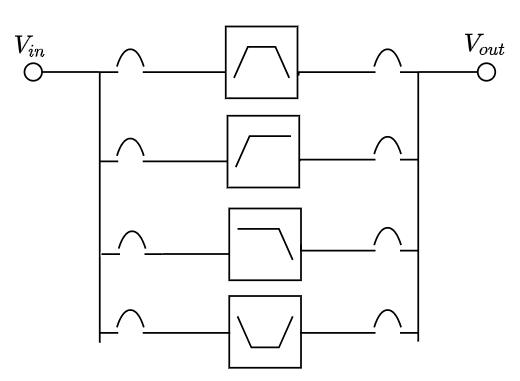
\includegraphics[width=0.6\textwidth]{../Ejercicio2-DiseñoDeFiltros/Imagenes/logic_diagram.png}
    \caption{Diagrama de Bloques lógico}
\end{figure}

La implementación final del PCB se presenta a continuación.
\begin{figure}[H]
    \centering
    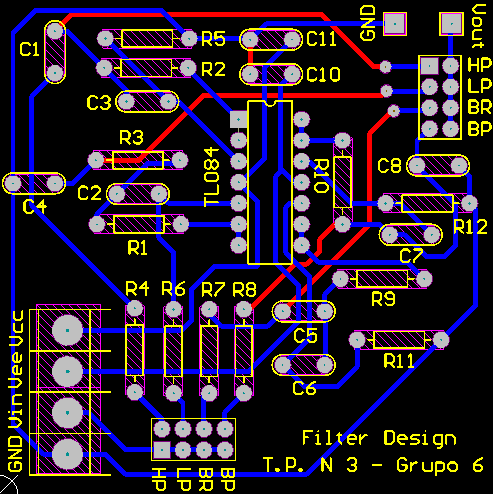
\includegraphics[width=0.6\textwidth]{../Ejercicio2-DiseñoDeFiltros/Imagenes/PCB_logic.png}
    \caption{Vista del PCB a nivel conexionado}
\end{figure}

\begin{figure}[H]
    \centering
    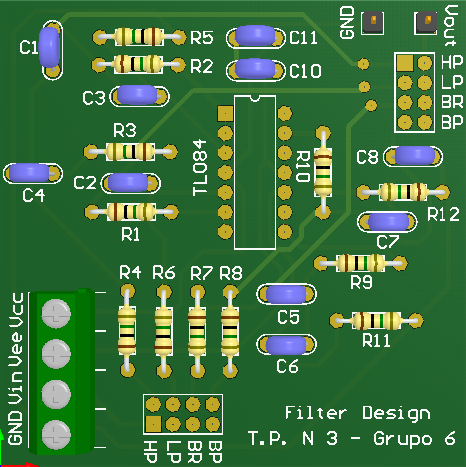
\includegraphics[width=0.6\textwidth]{../Ejercicio2-DiseñoDeFiltros/Imagenes/PCB_logic_3d.png}
    \caption{Vista 3D del PCB}
\end{figure}


La única consideración a realizar es que se omitió la utilización de agujeros de sujeción para colocar tamecos a la placa. Se decidió omitirlos 
para poder presentar el diseño de manera más clara y tener más espacio para pistas. Sin embargo, en una implementación real es indispensable tenerlos 
en consideración por comodidad y para una correcta manipulación del PCB.